\documentclass[10pt,a4paper,twoside]{article}
\usepackage[utf8]{inputenc}
\usepackage[francais]{babel}
\usepackage[T1]{fontenc}

%\usepackage{minted}
\usepackage{amsmath}
\usepackage{amsfonts}
\usepackage{amssymb}
\usepackage{graphicx}
%\usepackage{placeins}
%\usepackage{lscape}

%\usepackage{slashbox}


\author{Victor Lezaud}
\title{TD de probas - 3IF}
\begin{document}
\renewcommand{\partname}{Séance de Travaux Dirigés}

\maketitle
\renewcommand{\contentsname}{Sommaire}
\setcounter{tocdepth}{1}
\tableofcontents

\newpage
\part{Dénombrement - probabilités élémentaires}
\section{Jeu de carte}
On appelle main tout ensemble de 13 cartes prises dans un jeu de 52 cartes.
\subsection{Combien y a-t-il de mains différentes ?}
Il s'agit de prendre 13 cartes dans un jeu de 52 cartes sans remises et où l'ordre n'a aucune importance. Il s'agit donc de combinaisons sans remise de 13 éléments parmi 52. La réponse est donc :
\begin{align*}
N & =C_{52}^{13}\\
  & =\frac{52!}{13!(52-13)!}\\
  & =\frac{52!}{13!\times 39!}
\end{align*}

\subsection{Combien y a-t-il de mains contenant :}
\subsubsection{Au moins un pique ?}
Il s'agit de prendre une carte parmi les piques puis 12 cartes parmi les cartes restantes, l'ordre n'a aucune importance. Il s'agit donc de combinaison sans remise de 1 parmi 4 puis de 12 parmi 51. La réponse est donc :
\begin{align*}
N & = C^{1}_{4} \times C^{12}_{51}\\
  & = \frac{4!}{3! \times 1!} \times \frac{51!}{12! \times (51-12)!}\\
  & = 4\times\frac{51!}{13! \times 39!}
\end{align*}

\subsubsection{Au plus un pique ?}
Il s'agit de prendre 12 cartes parmi les cartes non piques puis 1 carte parmi les restantes, l'ordre n'a aucune importance. Il s'agit donc de combinaison sans remise de 12 parmi 39 puis de 1 parmi 40. La réponse est donc :
\begin{align*}
N & = C^{12}_{39} \times C^{1}_{40}\\
  & = \frac{39!}{12!\times (39-12)!} \times \frac{40!}{39!\times (40-39)!}\\
  & = 40 \times \frac{39!}{12!\times 27!}
\end{align*}

\subsubsection{Exactement 1 as et contenant au plus 2 piques}
Dans cette question nous allons étudier deux cas différents :
\begin{itemize}
\item[\textit{L'as est l'as de pique :}] Nous avons donc une carte fixée puis on tire 11 cartes parmi les non-piques non-as puis une carte parmi celles restantes non-as. Il s'agit donc de combinaison sans remise de 11 parmi 36 puis de 1 parmi 37. Cela donne:
\begin{align*}
N_{1} & = C^{11}_{36} \times C^{1}_{37}\\
  & = 37\times \frac{36!}{11!\times 25!}\\
\end{align*}
\item[\textit{L'as n'est pas un pique :}] L'as offre donc encore 3 choix possible. Ensuite on choisit 10 cartes parmi les non-piques non-as puis 2 cartes parmi les non-as restant. Il s'agit donc de combinaison sans remise de 1 parmi 3 puis de 10 parmi 36 puis de 2 parmi 38. 
\begin{align*}
N_{2} & = C^{1}_{3}\times C^{10}_{36} \times C^{2}_{38}\\
      & = \frac{3!}{2! \times 1!} \times \frac{36!}{10! \times 26!} \times \frac{38!}{2! \times 36!}\\
      & = 3 \times \frac{36!}{10! \times 26!} \times \frac{38!}{2\times 36!}
\end{align*}
\end{itemize}
L'ensemble des mains vérifiant le critère est l'union des ensembles des main correspondant à chacun des cas ainsi la réponse est :
$$N = N_{1}+N_{2}$$

\section{Lancer de dés 1}
\subsection*{Enoncé} 
Jacques dit à Paul : "si j'ai une chance sur six d'obtenir un six en lançant un dé, alors de double mes chances en le lançant deux fois". Jacques a-t-il raison ? Pourquoi ? (Construire un modèle probabiliste et traduire la question posée en termes de calcul de la probabilité d'un événement).

\subsection*{Réponse}
Jacques propose ici deux expériences aléatoires différentes
\subsection{Un lancer}
Dans cette première expérience on lance un dé équilibré. Ainsi l'univers est l'ensemble $\Omega = \{1,2,3,4,5,6\}$. On prend la tribu $T$ définie comme $T=P(\Omega)$. Comme le dé est équilibré on prend la probabilité $P:A\in \Omega \mapsto \frac{1}{card(\Omega)}$ avec $card(\Omega)=6$. Le triplet $(\Omega,T,P)$ forme donc un espace probabilisé. Nous étudions maintenant l'événement $A\in T$, avoir un 6. 
\begin{align*}
 & A=\{\omega\in\Omega, \omega=6\}\\ 
\Leftrightarrow & A=\{6\}\\
\Rightarrow & card(A)=1\\
\Rightarrow & P(A)=\frac{1}{6}
\end{align*}
Sur ce point Jacques a raison il a bien 1 chance sur 6 d'obtenir un 6 sur un lancer.

\subsection{Deux lancers}
Dans cette deuxième expérience on lance deux fois un dé équilibré. Ainsi l'univers est l'ensemble $\Omega' = \{(x,y), x\in \{1,\ldots,6\}\text{ et }y\in \{1,\ldots,6\}\}$. On prend la tribu définie comme $T'=P(\Omega')$. Comme le dé est équilibré on prend la probabilité $P':A\in \Omega' \mapsto \frac{1}{card(\Omega')}$ avec $card(\Omega')=36$. Le triplet $(\Omega',T',P')$ forme donc un espace probabilisé. Nous étudions maintenant l'événement $A'\in T'$, avoir au moins un 6.
\begin{align*}
 & A=\{(x,y)\in\Omega, x=6\text{ ou }y=6\}\\ 
\Leftrightarrow & A=\{(1,6),(2,6),(3,6),(4,6),(5,6),(6,6),(6,5),(6,4),(6,3),(6,2),(6,1)\}\\
\Rightarrow & card(A)=11\\
\Rightarrow & P(A)=\frac{11}{36}
\end{align*}
Jacques a donc 11 chances sur 36 d'obtenir un 6 sur deux lancers or
$$\frac{11}{36} < \frac{2}{6}$$
Donc Jacques à tort il ne double pas ses chances d'avoir un six en lançant deux fois le dé.

\section{Lancer de dés 2}
\subsection*{Enoncé}
Le prince de Toscane demande un jour à Galilée : pourquoi lorsqu'on jette 2 dés obtient-on plus souvent la somme 7 que la somme 6, bien que ces deux sommes soient obtenues de trois façons différentes ? (même indication)

\subsection*{Réponse}
Dans cette deuxième expérience on lance deux dés équilibrés. Ainsi l'univers est l'ensemble $\Omega = \{(x,y), x\in \{1,\ldots,6\}\text{ et }y\in \{1,\ldots,6\}\}$. On prend la tribu définie comme $T=P(\Omega)$. Comme le dé est équilibré on prend la probabilité $P:A\in \Omega \mapsto \frac{1}{card(\Omega)}$ avec $card(\Omega)=36$. Le triplet $(\Omega',T',P')$ forme donc un espace probabilisé. On s'intéresse ici aux deux événements $A\in T$, la somme des dés vaut 7 et $B\in T$ la somme des dés vaut 6.
\begin{align*}
  & A=\{(x,y)\in \Omega, x+y=7\}\\
\Leftrightarrow & A=\{(1,6),(2,5),(3,4),(4,3),(5,2),(6,1)\}\\
\Rightarrow & card(A) = 6\\
\Rightarrow & P(A) = \frac{6}{36} = \frac{1}{6}\\
\\
& B=\{(x,y)\in \Omega, x+y=6\}\\
\Leftrightarrow & B=\{(1,5),(2,4),(3,3),(4,2),(5,1)\}\\
\Rightarrow & card(B) = 5\\
\Rightarrow & P(B) = \frac{5}{36}
\end{align*}  
On remarque bien qu'il est plus probable d'avoir une somme égale à 7 qu'une somme égale à 6. Pour répondre au prince, cela est du au fait que 6 issues de l'expérience vérifie la condition de la somme égale à 7 contre seulement 5 pour la somme égale à 6.

\section{Anniversaire communs}
\subsection*{Enoncé}
Dans un groupe de $n$ personnes, quelle est la probabilité pour que les anniversaires de deux au moins d'entre elles tombent le même jour ?

\subsection*{Réponse}
Pour trouver la probabilité de l'événement $A_{n}$ au moins deux personnes ont le même anniversaire on étudie l'événement $A_{n}^{c}$ toutes les anniversaires sont différents. Dans notre étude l'univers est l'ensemble des $n$-uplets d'entier entre 1 et 365. Ainsi on a $card(\Omega)=365^{n}$. Et on suppose que chaque date a la même chance d'être une date d'anniversaire. La probabilité de $A$ peut-être calculé par :
\[ P(A_{n}) = 1-\frac{card(A_{n}^{c})}{365^{n}} \]
Ou $A_{n}^{c}$ est l'ensemble des dispositions ordonnées (car notre univers est ordonnée, mais l'exercice peut-être fait sans ordonnancement) de $n$ entiers entre 1 et 365. On a donc des arrangements sans remise ainsi :
\begin{align*}
card(A_{n}^{c}) &= A^{n}_{365}\\
 & = \frac{365!}{(365-n)!}
\end{align*}
ainsi on trouve $P(A_{n})$
\begin{align*}
P(A_{n}) & =1-\frac{\frac{365!}{(365-n)!}}{365^{n}}\\
  & = 1-\frac{365!}{(365-n)!\times 365^{n}}
\end{align*}


\section{Les deux enfants}
\subsection*{Enoncé}
Une famille a deux enfants. Quelle est la probabilité que ce soient deux garçons, sachant que le premier est un garçon ? Quelle est la probabilité que ce soient deux garçons sachant que l'un des deux au moins est un garçon ?

\subsection*{Réponse}
Soit $\Omega = \{(F,F),(F,G),(G,F),(G,G)\}$ un univers, $T=P(\Omega)$ une tribu et $P:\omega \in\Omega \mapsto \frac{1}{card(\Omega)}$ une probabilité, le triplet $(\Omega,T,P)$ forme un espace probabilisé modélisant notre problème. Soit $A$ l'événement avoir deux garçons, $B$ l'événement le premier est un garçon et $C$ l'événement il y a au moins un garçon, on obtient 
\begin{align*}
A & =\{(G,G)\} & B &=\{(G,F),(G,G)\} & C &=\{(F,G),(G,F),(G,G)\}\\
P(A) &=\frac{card(A)}{card(\Omega} & P(B) &=\frac{card(B)}{card(\Omega} & P(C) &=\frac{card(C)}{card(\Omega)}\\
P(A) &=\frac{1}{4} & P(B) &=\frac{2}{4} & P(C) &=\frac{3}{4}
\end{align*}
On cherche donc à calculer les probabilités de $A$ sachant $B$ et de $A$ sachant $C$. On étudie donc $A\cap B$ et $A\cap C$ or $A\subset B\subset C$ ainsi $A\cap B = A\cap C = A$, on obtient donc :
\begin{align*}
P(A|B) &= \frac{P(A\cap B)}{P(B)} & P(A|C) &= \frac{P(A\cap C)}{P(C)}\\
P(A|B) &= \frac{P(A)}{P(B)} & P(A|C) &= \frac{P(A)}{P(C)}\\
P(A|B) &= \frac{1}{2} & P(A|C) &= \frac{1}{3}
\end{align*}

\section{Le paquet de papillotes}
\subsection*{Enoncé}
Dans un paquet de papillotes, il y a 50 papillotes, dont 20 sont des pâtes de fruit, 20 sont au chocolat noir et 10 au chocolat au lait. Je pioche au hasard 4 papillotes. Quelle est la probabilité d'avoir 2 papillotes au chocolat au lait ? Combien en moyenne vais-je piocher de chocolat au lait ?

\subsection{Avoir 2 papillotes au chocolat au lait}
Soit $X$ la variable aléatoire réelle qui à un événement avoir $n$ papillotes au chocolat au lait associe l'entier $n$. On étudie l'événement $X\geqslant 2$. On travaille dans un espace probabilisé $(\Omega,T,P)$ avec $P:\omega\in\Omega\mapsto\frac{1}{card(\Omega)}$, on obtient donc :
$$P(X\geqslant2)=\frac{card(X\geqslant2)}{card(\Omega)}$$
L'univers $\Omega$ est l'ensemble des dispositions non ordonnées de 4 papillotes parmi 50 et $X\geqslant2$ est l'ensemble des dispositions non ordonnées de 2 papillotes au chocolat au lait parmi les 10 et de 2 papillotes parmi celles restantes. On obtient donc :
\begin{align*}
card(\Omega) &=C^{4}_{50} & card(X\geqslant2)&=C^{2}_{10}\times C^{2}_{48} 
\end{align*}
Ce qui nous donne :
\[ P(X\geqslant2)=\frac{C^{2}_{10}\times C^{2}_{48}}{C^{4}_{50}} \]

\subsection{Moyenne des papillotes au chocolat au lait}
(On attend ici un raisonnement intuitif, pas d'utilisation de la loi sous-jacente)\\
Une papillote sur 5 est au chocolat au lait donc sur 4 papillotes on obtient la moyenne $m=4*\frac{1}{5} = 0,8$

\newpage
\part{Probabilités élémentaires}
\setcounter{section}{0}

\section{Lancer de pièce}
\subsection*{Enoncé}
Soient $A$, $B$ et $C$ les événements correspondant au lancer de deux pièces équilibrées et distinguables suivants :
\begin{itemize}
\item $A$ = "La première pièce est tombée sur pile"
\item $B$ = "La deuxième pièce est tombée sur pile"
\item $C$ = "Les deux pièces sont tombées sur des faces différentes"
\end{itemize}

\subsection{Montrer que A,B et C sont deux à deux indépendants}
Soit $\Omega = \{(F,F),(F,P),(P,F),(P,P)\}$ un univers, $T=P(\Omega)$ une tribu sur cet univers et $P:\omega\in\Omega \mapsto \frac{1}{card(\Omega)}$ une probabilité, le triplet $(\Omega,T,P)$ forme un espace probabilisé modélisant l'expérience aléatoire du lancer de deux pièces équilibrées et distinguables. On a bien $(A,B,C)\in T^{3}$. On définit donc les événements $A$, $B$ et $C$ comme ceci :
\begin{align*}
A & = \{(x,y)\in \Omega, x=P\} & B & = \{(x,y)\in \Omega, y=P\} \\
A &= \{(P,F),(P,P)\} & B &= \{(F,P),(P,P)\}\\
P(A) &= \frac{2}{4} & P(B) &= \frac{2}{4}\\
P(A) &= \frac{1}{2} & P(B) &= \frac{1}{2}\\
\\
C & = \{(x,y)\in \Omega, x\neq y\}\\
C &=\{(F,P),(P,F)\}\\
P(C) &= \frac{2}{4}\\
P(C) &= \frac{1}{2}\\
\\
A\cap B &= \{(P,P)\} & A\cap C &= \{(P,F)\}\\
P(A\cap B)&=\frac{1}{4} & P(A\cap C)&=\frac{1}{4}\\
P(A\cap B)&=P(A)\times P(B) & P(A\cap C)&=P(A)\times P(C)\\
\\
B\cap C &= \{(F,P)\}\\
P(B\cap C)&=\frac{1}{4}\\
P(B\cap C)&=P(B)\times P(C)\\
\end{align*}
Les événements $A$, $B$ et $C$ sont bien deux à deux indépendants

\subsection{Sont-ils mutuellement indépendants ?}
On étudie l'événement $A\cap B\cap C$ :
\begin{align*}
A\cap B \cap C &= \{(P,F),(P,P)\} \cap \{(F,P),(P,P)\} \cap \{(F,P),(P,F)\}\\
A\cap B \cap C &= \emptyset\\
P(A\cap B \cap C) &= 0\\
P(A\cap B \cap C) &\neq P(A) \times P(B) \times P(C)
\end{align*} 
Les événements $A$, $B$ et $C$ ne sont pas mutuellement indépendants


\section{DS 2000}
\subsection*{Enoncé}
Un entrepôt est muni d'un dispositif d'alarme. Lorsqu'il y a tentative de cambriolage, le dispositif se déclenche avec une probabilité égale à 0,99. Lorsqu'il n'y a pas de tentative de cambriolage, le dispositif se déclenche tout de même par erreur au cours d'une journée égale à 0,01. En supposant qu'une tentative de cambriolage au cours d'une journée ait lieu avec une probabilité égale à 0,001, quelle est la probabilité qu'une alarme déclenchée un jour le soit par une tentative de cambriolage ?\\
On notera $D$ l'événement "l'alarme se déclenche" et $T$ l'événement "il y a une tentative de cambriolage", le tout considéré au cours de la journée donnée.
\subsection*{Réponse}
On cherche $P(T|D)$ la probabilité de $T$ sachant $D$ à partir de $P(D|T)$, $P(D|T^{c})$ et $P(T)$.
\begin{align*}
P(T|D) &=\frac{P(T\cap D)}{P(D)}\\
&= \frac{P(D|T)\times P(T)}{P(D|T)\times P(T) + P(D|T^{c}) \times P(T^{c})}\\
&= \frac{0,99 \times 0,001}{0,99\times 0,001 + 0,01 \times 0,999}\\
&\simeq 9\%
\end{align*}
La probabilité que l'alarme ait été déclenché par un cambriolage est de 9\%.

\section{Le minibus}
Un minibus-navette peut recevoir jusqu'à 5 passagers par voyage. La compagnie de transport accepte au maximum 6 réservations par voyage, chaque passager devant avoir une réservation. L'expérience antérieure a permis d'évaluer que 25\% des personnes effectuant une réservation ne se présentent pas au départ du voyage. Tous les passagers sont supposés agir indépendamment les uns des autres. On suppose pour toutes les questions que 6 réservations ont été faites

\subsection{Quelle est la probabilité qu'au moins un passager ayant réservé ne se présente pas au départ ?}
Soit $A$ l'événement : "Au moins un passager ayant réservé ne se présente pas au départ". $A^{c}$ est donc : "Tous les passagers ayant réservés se sont présentés". Or chaque passager a indépendamment 75\% de chance de se présenter ainsi on trouve :
\begin{align*}
P(A) &= 1-P(A^{c})\\
P(A) &= 1-0,75^{6}\\
P(A) &\simeq 0,82
\end{align*}

\subsection{Quel est le nombre moyen de passagers se présentant au départ ?}
Chaque passager a indépendamment 75\% de chance de se présenter ainsi on trouve une moyenne $m_{p}$ :
\[ m_{p}=6\times 0,75 = 4,5\]

\subsection{Quel est le nombre moyen de personnes transportées ?}
Tant qu'il manque au moins une personne le nombre de personne est égal au nombre de transporté. Il faut juste enlever 1 personne quand ils se sont tous présentés. Ainsi on trouve une moyenne $m_{t}$ :
\[ m_{t}=m_{p}-1\times P(A^{c}) = 4,5 - 0,18 = 3,32 \]

\section{Problème d'optimisation}
\subsection*{Enoncé}
On cherche à analyser le résultat d'un problème d'optimisation. Le programme de résolution a une probabilité $p$ de converger vers la valeur cherchée. On note $X$ le nombre d'essais nécessaires pour obtenir $m$ succès. On suppose les essais indépendants

\subsection{Pour tout $k\in\mathbb{N}$ déterminer la probabilité que $X=k$}
Si $X=k$ cela signifie que l'on a eu $m$ succès et $k-m$ échecs. Il faut donc avoir $k\geqslant m$. On trouve les probabilités suivante :
\begin{align*}
P(X=k)=\left\lbrace
\begin{array}{ll}
0 & \text{si } k\leq m\\
C^{m}_{k} \times m^{p} \times k^{1-p} & \text{sinon}
\end{array}\right.
\end{align*}

\subsection{Quel est le nombre moyen d'essais à effectuer pour obtenir $m$ succès}
En moyenne sur $n$ tirages il y a $np$ succès, donc pour avoir $m$ succès il faut en moyenne $\frac{m}{p}$ succès.

\newpage
\part{Variables aléatoires, espérance, variance}
\setcounter{section}{0}
\section{Loi de Poisson}
\subsection*{Enoncé}
Soit $X$ une variable aléatoire suivant une loi de Poisson $P(\lambda)$ avec $\lambda > 0$, c'est-à-dire telle que
\[ P(X=k)=C(\lambda)\frac{\lambda^{k}}{k!}  \]
Cette loi est utilisée notamment pour modéliser les phénomènes de files d'attentes, par exemple $X$ est le nombre de requêtes sur un serveur informatique par minutes.

\subsection{Expliciter $C(\lambda)$ en fonction de $\lambda$}
Pour une variable aléatoire réelle $X$ suivant une loi de Poisson on a :
\[P(X=k) = e^{-\lambda}\frac{\lambda^{k}}{k!} \]
Donc par identification on a :
\[ C(\lambda) = e^{-\lambda} \]

\subsection{Calculer la fonction génératrice de $X$, qu'on notera $G_{X}$}
\begin{align*}
G_{X}(s) &= E(s^{X})\\
 &= \sum_{n\in\mathbb{N}}s^{n} \times P(X=n)\\
 &= \sum_{n\in\mathbb{N}}s^{n} \times e^{-\lambda} \frac{\lambda^{n}}{n!}\\
 &= e^{-\lambda}\sum_{n\in\mathbb{N}} \frac{(\lambda s)^{n}}{n!}\\
 &= e^{-\lambda}\times e^{\lambda s}\\
G_{X}(s) &= e^{\lambda(s-1)}\\
\end{align*}

\subsection{Sachant que $G_{X}'(1)=E(X)$ et que $G_{X}''(1)=E(X(X-1))$, en déduire $E(X)$ puis $Var(X)$.}
On a $G_{X}(s) = e^{\lambda(s-1)}$ ainsi on obtient $G_{X}'(s) =\lambda e^{\lambda(s-1)}$ et $G_{X}''(s) =\lambda^{2} e^{\lambda(s-1)}$
\begin{align*}
E(X) &= G_{X}'(1)\\
&= \lambda e^{\lambda(1-1)}\\
&= \lambda e^{0}\\
E(X) &= \lambda\\
\\
Var(X) &= E(X^{2})-E(X)^{2}\\
&= E(X^{2}-X+X)-E(X)^{2}\\
&= E\left(X(X-1)\right() + E(X) - E(X)^{2}\\
&= G_{X}''(1) - E(X)^{2} + E(X)\\
&= \lambda^{2} - \lambda^{2} + \lambda\\
Var(X) &= \lambda\\
\end{align*}

\section{Les caisses du magasins}
\subsection*{Enoncé}
Dans un magasin pourvu de deux caisses, on note $X$ et $Y$ le nombre de personnes passant respectivement à la première et à la deuxième caisse dans un intervalle de temps de 30 minutes. On suppose que ces deux v.a. sont indépendantes et suivent des lois de Poisson de paramètres respectifs $\lambda$ et $\mu$.
\subsection{Quelle est la loi du nombre de personnes passant aux deux caisses, $X+Y$ ?}
Les variables aléatoires $X$ et $Y$ suivent une loi de Poisson de paramètres respectif $\lambda$ et $\mu$. Donc soit $G_{X}$ et $G_{Y}$ on a :
\begin{align*}
G_{X}(s) = e^{\lambda(s-1)} && G_{y}(s) = e^{\mu(s-1)}\\
\end{align*}
Soit $G_{X+Y}$ la fonction génératrice de la variable aléatoire $X+Y$, on a:
\begin{align*}
G_{X+Y}(s) &= G_{X}(s) \times G_{Y}(s)\\
 &= e^{\lambda(s-1)} \times e^{\mu(s-1)}\\
G_{X+Y}(s) &= e^{(\lambda+\mu)(s-1)} \\
\end{align*}
On reconnaît la fonction génératrice d'une loi de Poisson. La variable aléatoire $X+Y$ suit donc une loi de Poisson de paramètre $\lambda+\mu$

\subsection{Loi conditionnelle}
\subsubsection*{Question}
Le gérant m'assure que le débit est constant avec les deux caisses et que $X+Y=k$, avec $k\in\mathbb{N}$. J'ai choisi la file de la première caisse. J'aimerais donc connaître la loi conditionnelle de $X$ sachant $X+Y=k$. Déterminer cette loi.

\subsubsection*{Réponse}
On calcule la probabilité de $X=l$ avec $l\in\mathbb{N}$ sachant $X+Y=k$
\begin{align*}
P(X=l|X+Y=k) &= \frac{P(X=l\cap X+Y=k)}{P(X+Y=k)}\\
&= \frac{P(X=l \cap Y=k-l)}{P(X+Y=k)}\\
&= \frac{P(X=l)\times P(Y=k-l)}{P(X+Y=k)} & \text{par indépendance}\\
&= \frac{e^{-\lambda}\frac{\lambda^{l}}{l!}\times e^{-\mu}\frac{\mu^{k-l}}{(k-l)!}}{e^{-\lambda-\mu}\frac{(\lambda+\mu)^{k}}{(k)!}}\\
&= \frac{\frac{\lambda^{l}\mu^{k-l}}{(k-l)!\times l!}}{\frac{(\lambda+\mu)^{k}}{k!}}\\
&=\frac{k!}{(k-l)!\times l!} \times \frac{\lambda^{l}}{(\lambda+\mu)^{l}} \times \frac{\mu^{k-l}}{(\lambda+\mu)^{k-l}} \\
&=C^{l}_{k}\times\left(\frac{\lambda}{\lambda+\mu}\right)^{l}\times\left(\frac{\mu}{\lambda+\mu}\right)^{k-l}\\
P(X=l|X+Y=k) &=C^{l}_{k}\times\left(\frac{\lambda}{\lambda+\mu}\right)^{l}\times\left(1-\frac{\lambda}{\lambda+\mu}\right)^{k-l}\\
\end{align*}
On reconnaît une loi binomiale avec $k$ épreuves de probabilités de succès $\frac{\lambda}{\lambda+\mu}$. On a donc $X+Y \sim B(k,p)$ avec $p=\frac{\lambda}{\lambda+\mu}$.

\section{DS 2003}
\subsection*{Enoncé}
On modélise le temps CPU requis par une tâche classique par une variable aléatoire positive $X$ dont la loi (appelée loi hyperexponentielle) est définie de la façon suivante :
\[\forall t\geqslant0,\ P(X\leqslant t)=\alpha(1-e^{-\lambda_{1}t})+(1-\alpha)(1-e^{-\lambda_{2}t}) \]

\subsection{Calculer la densité de $X$}
Soit $F_{X}$ la fonction de répartition de $X$ et $f_{X}$ sa densité. On a $f_{X}(t) = F_{X}'(t)$ avec $F_{X}(t) = P(X\leqslant t)$. Ainsi :
\begin{align*}
f_{X}(t) &= \alpha\lambda_{1} e^{-\lambda_{1}t} + (1-\alpha)\lambda_{2} e^{-\lambda_{2}t}\\
\end{align*}

\subsection{Calculer le temps CPU moyen $E(X)$}
\begin{align*}
E(X) &= \int_{\mathbb{R^{+}}} t \times P(X=t) dt\\
&= \int_{\mathbb{R^{+}}} t(\alpha\lambda_{1} e^{-\lambda_{1}t} + (1-\alpha)\lambda_{2} e^{-\lambda_{2}t})dt\\
&= \alpha\lambda_{1} \int_{\mathbb{R^{+}}}te^{-\lambda_{1}t}dt+(1-\alpha)\lambda\int_{\mathbb{R^{+}}}te^{-\lambda_{2}t}dt & \text{or }\int_{\mathbb{R^{+}}}te^{-\lambda t}dt = \frac{1}{\lambda^{2}}\\
E(X) &= \frac{\alpha}{\lambda_{1}}+\frac{1-\alpha}{\lambda_{2}}\\
\end{align*}

\subsection{Calculer $Var(X)$}
\begin{align*}
E(X^{2}) &= \int_{\mathbb{R^{+}}} t^{2} \times P(X=t) dt\\
&= \int_{\mathbb{R^{+}}} t^{2}(\alpha\lambda_{1} e^{-\lambda_{1}t} + (1-\alpha)\lambda_{2} e^{-\lambda_{2}t})dt\\
&= \alpha\lambda_{1} \int_{\mathbb{R^{+}}}t^{2}e^{-\lambda_{1}t}dt+(1-\alpha)\lambda\int_{\mathbb{R^{+}}}t^{2}e^{-\lambda_{2}t}dt & \text{or }\int_{\mathbb{R^{+}}}t^{2}e^{-\lambda t}dt = \frac{2}{\lambda^{3}}\\
E(X^{2}) &= \frac{2\alpha}{\lambda_{1}^{2}}+\frac{2(1-\alpha)}{\lambda_{2}^{2}}\\
\\
Var(X) &= E(X^{2})-E(X)^{2}\\
&= \frac{2\alpha}{\lambda_{1}^{2}}+\frac{2(1-\alpha)}{\lambda_{2}^{2}} - \left(\frac{\alpha}{\lambda_{1}}+\frac{1-\alpha}{\lambda_{2}}\right)^{2}\\
\end{align*}

\section{Algorithme de simulation}
\subsection*{Enoncé}
Soit $X$ une variable aléatoire à valeurs dans $\{-1,0,1\}$ telle que $P(X=-1)=\frac{1}{3}$, $P(X=0)=\frac{1}{2}$ et $P(X=1)=\frac{1}{6}$. Proposer un algorithme de simulation de $X$. On supposera qu'on sait simuler une variable aléatoire de loi uniforme sur $[0,1]$.

\subsection*{Réponse}
On simule une variable aléatoire de loi uniforme sur $[0,1]$ et on stocke la valeur dans une variable $y$.
\begin{itemize}
\item si $y<\frac{1}{3}$ alors $X=-1$
\item sinon si $y<\frac{5}{6}$ alors $X=0$
\item sinon $X=1$
\end{itemize}

\newpage
\part{Variables aléatoires continues}
\setcounter{section}{0}
\section{Note et loi normale}
La note obtenu par des étudiants à un examen est une v.a.r. normale $X\sim N(7,3^{2})$
\subsection{Note supérieur à 10}
\paragraph{Question :} Calculer le pourcentage d'individus ayant plus de 10.

\paragraph{Réponse :} On utilise le tableau de valeurs de la loi normale $N(0,1)$. Avoir plus de 10 pour la loi $N(7,3^{2})$ équivaut à avoir plus de 1 pour la loi $N(0,1)$. On a environ 16\% de note supérieure ou égale à 10.

\subsection{Les pires 10\%}
\paragraph{Question :} Calculer la note en dessous de laquelle se trouvent 10\% des étudiants.

\paragraph{Réponse :} On utilise le tableau de valeurs de la loi normale $N(0,1)$. Selon cette loi 10\% des valeurs sont en-dessous de -1,28 soit $m-1,28\sigma$. Or pour $N(7,3^{2})$, $m-1,28\sigma=3,4$. On a donc 10\% des élèves ont en-dessous de 3,4.

\subsection{Revalorisation des notes}
\paragraph{Question :} Compte tenu des résultats obtenus, on décide de revaloriser l'ensemble des notes par une transformation linéaire $Z=aX+b$. Quelles valeurs doit-on donner à $a$ et $b$ pour que les valeurs précédentes passent respectivement à 50\% et 7 ?

\paragraph{Réponse :} On veut $E(Z)=10$ et $Var(Z) = (\frac{10-7}{1,28})^{2} = 2,34^{2}$ or on a $a=\frac{\sigma_{Z}}{\sigma_{X}}$ et $b=E(Z)-aE(X)$ ainsi :
\begin{align*}
a&=\frac{2,34}{3} &  b&=10-7a\\
&=0,78 & &=4,53
\end{align*}

\section{Loi log-normale}
\subsection*{Enoncé}
On dit qu'une variable aléatoire réelle $Y$ suit une loi log-normale si $Y=e^{X}$ avec $X\sim N(m,\sigma^{2})$. Calculer l'espérance d'une loi log-normale.

\subsection*{Réponse}
\begin{align*}
E(Y) & = E\left( e^{X} \right)\\
&= \int_{\mathbb{R}} e^{t} \times P(X=t) dt\\
&= \int_{\mathbb{R}} e^{t} \frac{1}{\sqrt{2\pi\sigma^{2}}} e^{-\frac{(t-m)^{2}}{2\sigma^{2}}} dt\\
&= \frac{1}{\sqrt{2\pi\sigma^{2}}} \int_{\mathbb{R}} e^{t-\frac{(t-m)^{2}}{2\sigma^{2}}} dt\\
\end{align*}
Notre but maintenant est de faire apparaître dans l'intégrale une fonction de densité $f_{Z}$ d'une variable aléatoire $Z$ qui suit une loi normale (de paramètres différents). Ainsi on saura que l'intégrale de cette fonction vaut 1. On se concentre sur le calcul à l'intérieur de l'exponentielle :
\begin{align*}
t-\frac{(t-m)^{2}}{2\sigma^{2}} &= \frac{2\sigma^{2}t-t^{2}+2tm-m^{2}}{2\sigma^{2}}\\
&= \frac{-t^{2}+2t(m+\sigma^{2})-m^{2}}{2\sigma^{2}}\\
\end{align*}
Ici on cherche à faire apparaître une somme au numérateur avec un terme de la forme $-(t-m')^{2}$ et un autre terme qui ne dépend pas de $t$. Ainsi on pourra sortir le 2e terme car c'est un facteur constant dans l'intégrale. Et le premier terme nous donnera une fonction de densité de la loi normale de paramètre $N(m',\sigma^{2})$. On a une forme proche de la version développée de $-(t-m')^{2}$ avec $m'=m+\sigma^{2}$. Il nous faudrait juste $(m+\sigma^{2})^{2}$ à la place de $m^{2}$. On le fait donc apparaître :

\begin{align*}
t-\frac{(t-m)^{2}}{2\sigma^{2}} &= \frac{-t^{2}+2t(m+\sigma^{2})-m^{2}-2m\sigma^{2}-\sigma^{4}+2m\sigma^{2}+\sigma^{4}}{2\sigma^{2}}\\
&= \frac{-t^{2}+2t(m+\sigma^{2})-(m+\sigma^{2})^{2}}{2\sigma^{2}}+\frac{2m\sigma+\sigma^{4}}{2\sigma^{2}}\\
&= \frac{-(t-(m+\sigma^{2}))^{2}}{2\sigma^{2}}+\frac{\sigma^{4}+2m\sigma^{2}+m^{2}-m^{2}}{2\sigma^{2}}\\
&= \frac{-(t-m-\sigma^{2})^{2}}{2\sigma^{2}} + \frac{(m+\sigma^{2})^{2}-m^{2}}{2\sigma^{2}}
\end{align*}
On a bien obtenu ce que l'on cherchait on peut maintenant réinjecter ce résultat dans le calcul précédent :
\begin{align*}
E(Y) & = \frac{1}{\sqrt{2\pi\sigma^{2}}} \int_{\mathbb{R}} e^{t-\frac{(t-m)^{2}}{2\sigma^{2}}} dt\\
&= \frac{1}{\sqrt{2\pi\sigma^{2}}} \int_{\mathbb{R}} e^{\frac{-(t^{2}-m-\sigma^{2})^{2}}{2\sigma^{2}}} \times e^{\frac{(m+\sigma^{2})^{2}-m^{2}}{2\sigma^{2}}} dt\\
&= e^{\frac{(m+\sigma^{2})^{2}-m^{2}}{2\sigma^{2}}} \times \int_{\mathbb{R}} \frac{1}{\sqrt{2\pi\sigma^{2}}} e^{\frac{-(t^{2}-m-\sigma^{2})^{2}}{2\sigma^{2}}} dt
\end{align*}
Soit $f_{Z}$ une fonction telle que $f_{Z}(t) = \frac{1}{\sqrt{2\pi\sigma^{2}}} e^{\frac{-(t^{2}-m-\sigma^{2})^{2}}{2\sigma^{2}}}$. Cette fonction est une fonction de densité d'une loi normale de paramètre $N(m+\sigma^{2},\sigma^{2})$ ainsi on sait que $\int_{\mathbb{R}}f_{Z}(t)dt = 1$.
\begin{align*}
E(Y) &= e^{\frac{(m+\sigma^{2})^{2}-m^{2}}{2\sigma^{2}}} \times \int_{\mathbb{R}}f_{Z}(t)dt\\
E(Y) &= e^{\frac{(m+\sigma^{2})^{2}-m^{2}}{2\sigma^{2}}}
\end{align*}

\section{Fonction caractéristique}
\subsection*{Enoncé}
Soit $X_{1},\ldots,X_{N}$ indépendantes de loi $N(0,1)$. Calculer la fonction caractéristique de $D^{2}=X_{1}^{2}+\ldots+X_{N}^{2}$

\subsection*{Réponse}
On calcule d'abord la fonction caractéristique d'une variable $X^{2}$ avec $X\sim N(0,1)$
\begin{align*}
\Phi_{X^{2}}(t) &= E\left(e^{itX^{2}}\right)\\
&= \int_{\mathbb{R}} e^{itx^{2}} \frac{1}{\sqrt{2\pi}} e^{-\frac{x^{2}}{2}} dx \\
&= \int_{\mathbb{R}} \frac{1}{\sqrt{2\pi}} e^{-(1-2it)\frac{x^{2}}{2}} dx\\
&= (1-2it)^{-\frac{1}{2}}\\
\end{align*}
$D^{2}$ est la somme de $N$ variables $X$ indépendantes de loi $N(0,1)$. Or la fonction caractéristique de la somme de variables aléatoires est le produits des fonctions caractéristiques de ces variables aléatoires. Ainsi on obtient :
\begin{align*}
D^{2} &= \sum_{i=1}^{N} X_{i}^{2}\\
\Phi_{D^{2}}(t) &= \prod_{i=1}^{N} \Phi_{X_{i}^{2}}(t) \\
 & = (\Phi_{X_{i}^{2}}(t))^{N} \\
 & = (1-2it)^{-\frac{N}{2}}\\
\end{align*}


\section{Loi exponentielle}
\subsection*{Enoncé}
Montrer que si $X\sim \varepsilon(\lambda)$, alors pour tous réels $a$ et $b$ positifs, on a :
\[ P(X>a+b \mid X>b) = P(X>a) \]

\subsection*{Réponse}
\begin{align*}
P(X>a) &= 1-P(X\leqslant a)\\
&= 1-\int_{0}^{a}\lambda e^{-\lambda t}dt\\
&= 1-\left[ -e^{-\lambda t} \right]_{0}^{a}\\
&= 1 + e^{-\lambda a} - 1\\
&= e^{-\lambda a}\\
\\
P(X>a+b|X>b) &= 1-P(X\leqslant a+b | X>b)\\
&= 1-\frac{P(X\leqslant a+b \cap X>b)}{P(X>b)}\\
&= 1- \frac{\int_{b}^{a+b} \lambda e^{-\lambda t} dt}{1-\int_{0}^{b}\lambda e^{-\lambda t}dt}\\
&= 1-\frac{\left[ -e^{-\lambda t} \right]_{b}^{a+b}}{1-\left[ -e^{-\lambda t} \right]_{0}^{b}}\\
&= 1 + \frac{e^{-\lambda(a+b)} - e^{-\lambda b}}{1 + e^{-\lambda b} - 1}\\
&= 1 + \frac{e^{-\lambda b} (e^{-\lambda a} - 1)}{e^{-\lambda b}}\\
&= 1 + e^{-\lambda a} - 1\\
&= e^{-\lambda a}\\
\\
P(X>a+b\mid X>b) &= P(X>a)
\end{align*}


%\section{Fonction de répartition}
%\subsection*{Enoncé}
%Soit $F$ la fonction de répartition d'une loi de probabilité. On pose pour tout $t\in [0,1],\ F^{-1}(t)=inf\{s,F(s)>t\}$. Cette fonction est bien définie grâce aux propriétés des fonctions de répartition. Soit $U$ une variable aléatoire de loi uniforme sur $[0,1]$. Quelle est la loi de $F^{-1}(U)$ ? A quoi peut servir ce résultat ?
%
%\subsection*{Réponse}
%\begin{align*}
%F(x) &= \left\lbrace\begin{array}{ll}
%0 & \text{si }x<a\\
%\frac{x-a}{b-a} & \text{si }a<x<b\\
%1 & \text{si }x>b\\
%\end{array}\right.\\
%F^{-1}(0) &= ]a,+\infty[\\
%F^{-1}(1) &= \emptyset\\
%F^{-1}(x) &= ]a+(b-a)x,+\infty[
%\end{align*}


\newpage
\part{Vecteurs aléatoires : Lois marginales, Indépendance, Loi conditionnelles}
\setcounter{section}{0}
\section{Couple de variable}
\subsection*{Enoncé}
On considère un couple de variables aléatoires $(X,Y)$ de densité :
\[ f_{(X,Y)}(x,y) = 
\left\lbrace \begin{array}{ll}
\frac{1}{x}e^{-x} & \text{si }0<y<x\\
0 & \text{sinon}
\end{array}\right.
\]

\subsection{Les v.a. $X$ et $Y$ sont-elles indépendantes ?}
Les variables aléatoires $X$ et $Y$ sont indépendantes si et seulement si on peut trouver leur densité $f_{X}$ et $f_{Y}$ telles que $f_{X}$ ne dépende pas de $Y$, $f_{Y}$ ne dépende pas de $X$ et $f_{(X,Y)}=f_{X}f_{Y}$. On trouve :
\begin{align*}
f_{X}(x) &= \int_{\mathbb{R}}f_{(X,Y)}(x,y) dy \\
&= \int_{0}^{x} \frac{1}{x}e^{-x} dy\\
&= \frac{1}{x}e^{-x} \times \int_{0}^{x}dy\\
&= \left\lbrace \begin{array}{ll}
e^{-x} & \text{si }0<x\\
0 & \text{sinon}
\end{array}\right.
\end{align*}
On cherche donc $f_{Y}$ ne dépendant pas de $X$ tel que $f_{Y}=\frac{f_{(X,Y)}}{f_{X}}$. On calcule donc :
\begin{align*}
\frac{f_{(X,Y)}}{f_{X}}(x,y) &= \left\lbrace \begin{array}{ll}
\frac{\frac{1}{x}e^{-x}}{e^{-x}} & \text{si }0<y<x\\
0 & \text{sinon}
\end{array}\right.\\
&= \left\lbrace \begin{array}{ll}
\frac{1}{x} & \text{si }0<y<x\\
0 & \text{sinon}
\end{array}\right.\\
\end{align*}
Cette fonction dépend de $x$, les variables $X$ et $Y$ ne sont donc pas indépendantes.

\subsection{Déterminer la loi marginale de $X$ puis la loi conditionnelle de $Y$ sachant $X$}
\subsubsection{Loi marginale de $x$}
\begin{align*}
f_{X}(x) &= \int_{\mathbb{R}}f_{(X,Y)}(x,y) dy \\
&= \int_{0}^{x} \frac{1}{x}e^{-x} dy\\
&= \frac{1}{x}e^{-x} \times \int_{0}^{x}dy\\
&= \left\lbrace \begin{array}{ll}
e^{-x} & \text{si }0<x\\
0 & \text{sinon}
\end{array}\right.
\end{align*}

\subsubsection{Loi conditionnelle de $Y$ sachant $X$}
Soit $f_{Y|X=x}$ la densité conditionnelle de $Y$ sachant $X$ :
\begin{align*}
f_{Y|X=x}(y) &= \frac{f_{(X,Y)}(x,y)}{f_{X}(x)}\\
&= \left\lbrace \begin{array}{ll}
\frac{\frac{1}{x}e^{-x}}{e^{-x}} & \text{si }0<y<x\\
0 & \text{sinon}
\end{array}\right.\\
&= \left\lbrace \begin{array}{ll}
\frac{1}{x} & \text{si }0<y<x\\
0 & \text{sinon}
\end{array}\right.
\end{align*}
La loi conditionnelle de $Y$ sachant $X$ est une loi uniforme sur l'intervalle $[0,x]$.

\section{Lancer de dés}
\subsection*{Enoncé}
On jette deux dés équilibrés. On désigne respectivement par $X$ et par $Y$ le maximum et le minimum des résultats obtenus.

\subsection{Déterminer la loi du couple $(X,Y)$}

\renewcommand\arraystretch{1.75}
\begin{tabular}{|c|cccccc|c|}
\hline 
 & 1 & 2 & 3 & 4 & 5 & 6 & loi marginale de $X$ \\ 
\hline 
1 & $\frac{1}{36}$ & 0 & \multicolumn{3}{c}{$\cdots$} & 0 & $\frac{1}{36}$ \\ 
2 & $\frac{2}{36}$ & $\frac{1}{36}$ & 0 & \multicolumn{2}{c}{$\cdots$} & 0 & $\frac{3}{36}$\\
3 & $\frac{2}{36}$ & $\frac{2}{36}$ & $\frac{1}{36}$ & 0 & $\cdots$ & 0 & $\frac{5}{36}$\\
4 & $\frac{2}{36}$ & $\frac{2}{36}$ & $\frac{2}{36}$ & $\frac{1}{36}$ & 0 & 0 & $\frac{7}{36}$\\
5 & $\frac{2}{36}$ & $\frac{2}{36}$ & $\frac{2}{36}$ & $\frac{2}{36}$ & $\frac{1}{36}$ & 0 & $\frac{9}{36}$\\
6 & $\frac{2}{36}$ & $\frac{2}{36}$ & $\frac{2}{36}$ & $\frac{2}{36}$ & $\frac{2}{36}$ & $\frac{1}{36}$ & $\frac{11}{36}$\\
\hline
loi marginale de $Y$ & $\frac{11}{36}$ & $\frac{9}{36}$ & $\frac{7}{36}$ & $\frac{5}{36}$ & $\frac{3}{36}$ & $\frac{1}{36}$ & 1\\
\hline
\end{tabular} 
\renewcommand\arraystretch{1}

\subsection{Les variables $X$ et $Y$ sont-elles indépendantes ?}
\begin{align*}
P(X=1) &= \frac{1}{36}\\
P(Y=1) &= \frac{11}{36}\\
P(X=1\cap Y=1) &= \frac{1}{36}\\
P(X=1)\times P(Y=1) &\neq P(X=1\cap Y=1)\\
\end{align*}
Les variables $X$ et $Y$ ne sont pas indépendantes.

\section{Reproduction des batraciens}
\subsection*{Enoncé}
On suppose que le nombre $N$ d'oeufs pondus par un batracien suit une loi de Poisson de paramètre $\lambda$. De plus, on suppose également que les oeufs pondus ont une évolution indépendantes les uns des autres, et que chaque oeuf a une probabilité $p$ d'arriver à éclosion. On note $X$ le nombre d'oeufs éclos.

\subsection{Déterminer la loi du couple aléatoire $(X,N)$}
$N$ suit une loi de Poisson de paramètre $\lambda$ on obtient donc :
\[ \forall n \in \mathbb{N}^{+}\ \ P(N=n)=e^{-\lambda}\frac{\lambda^{n}}{n!}   \]
L'éclosion d'un oeuf correspond à une épreuve de Bernoulli de paramètre $p$. Ainsi le nombre d'éclosions $N$ suit une loi binomiale de paramètre $(n,p)$. On obtient donc :
\[ \forall x \in \mathbb{N}^{+}\ \ P(X=x\mid N=n)= C_{n}^{x} (1-p)^{n-x} p^{x} \]
On obtient donc pour le couple $(X,Y)$ :
\begin{align*}
P(N=n\cap X=x) &= P(N=n) \times P(X=x|N=n)\\
&= e^{-\lambda}\frac{\lambda^{n}}{n!}  \times C_{n}^{x} (1-p)^{n-x} p^{x}\\
&= \frac{\lambda^{n}}{n!}\frac{n!}{x!(n-x)!} e^{-\lambda} p^{x} (1-p)^{n-x}\\
&= \frac{\lambda^{n}}{x!(n-x)!}e^{-\lambda} p^{x} (1-p)^{n-x}\\
\end{align*}

\subsection{En déduire la loi de $X$}
\begin{align*}
P(X=x) &= \sum_{n=0}^{+\infty} P(N=n \cap X=x)\\
&= \sum_{n=0}^{+\infty} \frac{\lambda^{n}}{x!(n-x)!}e^{-\lambda} p^{x} (1-p)^{n-x}\\
&= e^{-\lambda}\frac{p^{x}}{x!} \sum_{n=0}^{+\infty} \frac{\lambda^{n} (1-p)^{n-x}}{(n-x)!}\\
&= e^{-\lambda}\frac{p^{x}}{x!} \sum_{n=0}^{+\infty} \frac{\lambda^{n-x} \lambda^{x} (1-p)^{n-x}}{(n-x)!}\\
&= \frac{p^{x}\lambda^{x}}{x!} e^{-\lambda} \sum_{n=0}^{+\infty} \frac{(\lambda (1-p))^{(n-x)}}{(n-x)!}\\
&= \frac{p^{x}\lambda^{x}}{x!} e^{-\lambda} e^{\lambda(1-p)}\\
P(X=x) &= e^{-\lambda p} \frac{(\lambda p)^{x}}{x!}
\end{align*}
La variable aléatoire $X$ suit donc une loi de Poisson de paramètre $\lambda p$

\newpage
\part{Covariance - Théorèmes limites}
\setcounter{section}{0}
\section{Lancer de dé}
\subsection*{Enoncé}
Un dé équilibré est lancé $n$ fois de suite. Soient les événements $A_{i}=$"on obtient 1 au $i^{eme}$ lancer", et $B_{i}=$"on obtient 2 au $i^{eme}$ lancer". Soient alors les v.a.r. :
\begin{align*}
X_{i} = \left\lbrace \begin{array}{ll}
1 & \text{si }A_{i}\text{ est vérifié}\\
0 & \text{sinon}
\end{array}\right.
&&
Y_{i} = \left\lbrace \begin{array}{ll}
1 & \text{si }B_{i}\text{ est vérifié}\\
0 & \text{sinon}
\end{array}\right.
\end{align*} 
Soient $X$ et $Y$ les v.a.r. représentant respectivement le nombre de fois où on a obtenu 1 et le nombre de fois où on a obtenu 2 sur les $n$ lancers.


\subsection{Quelles sont les lois de $X_{i}$ et $Y_{i}$ ?}
Obtenir un chiffre précis sur un lancer de dé est une épreuve de Bernoulli avec une probabilité de succès de $\frac{1}{6}$. $X$ et $Y$ suivent donc des lois de Bernoulli de paramètre $\frac{1}{6}$ 
\begin{align*}
X_{i} \sim B\left(1,\frac{1}{6}\right) && Y_{i} \sim B\left(1,\frac{1}{6}\right)
\end{align*}

\subsection{Quelles sont les lois de $X$ et $Y$ ?}
$X$ est une v.a.r. qui compte le nombre de succès parmi les v.a.r. $X_{i}$. Il s'agit donc d'une v.a.r. qui comptent le nombre de succès parmi $n$ épreuve de Bernoulli identiques de paramètre $\frac{1}{6}$. $X$ suit donc une loi binomiale de paramètre $(n,\frac{1}{6})$. Il en va de même pour $Y$.
\begin{align*}
X \sim B\left(n,\frac{1}{6}\right) && Y \sim B\left(n,\frac{1}{6}\right)
\end{align*}

\subsection{Calculer $\rho(X,Y)$}
On définit le couple de variables $(X,Y)$ et on cherche son espérance :
\begin{align*}
E(X,Y) &= \sum_{i=1}^{n}\sum_{j=1}^{n} P(A_{i}\cap B_{j})\\
\end{align*}
Or $A_{i}$ et $B_{j}$ sont indépendant si $i\neq j$ car les lancers sont mutuellement indépendants et si $i=j$ alors $A_{i}\cap B_{j} = \emptyset$ car on ne peut avoir un 1 et un 2 sur un même lancer. On a donc :
\begin{align*}
E(X,Y) &= \sum_{i=1}^{n}\sum_{j=1}^{n} P(A_{i})\times P(B_{j}) - \sum_{k=1}^{n} P(A_{k})\times P(B_{k})\\
&= \sum_{i=1}^{n}\sum_{j=1}^{n} \frac{1}{6}\times \frac{1}{6} - \sum_{k=1}^{n} \frac{1}{6} \times \frac{1}{6}\\
&= n\times n\times \frac{1}{36} - n \times \frac{1}{36}\\
&= \frac{n(n-1)}{36}
\end{align*}
De plus on sait que $E(X)=E(Y)=\frac{n}{6}$. Ainsi on calcule $Cov(X,Y)$ :
\begin{align*}
Cov(X,Y) &= E(X,Y) - E(X) \times E(Y)\\
 & = \frac{n(n-1)}{36} - \frac{n}{6} \times \frac{n}{6}\\
 & = -\frac{n}{36}
\end{align*}
On cherche maintenant $Var(X)$ et $Var(Y)$. $X$ suit une loi binomiale composée de $n$ épreuve de Bernoulli de probabilité $\frac{1}{6}$. De même pour $Y$ ainsi on a :
\begin{align*}
Var(X) &= n\frac{1}{6}\left(1-\frac{1}{6}\right) & Var(Y) &= n\frac{1}{6}\left(1-\frac{1}{6}\right)\\
&= n\frac{1}{6}\times\frac{5}{6} & &= n\frac{1}\times{6}\frac{5}{6}\\
&= \frac{5n}{36} & &= \frac{5n}{36}
\end{align*}
On peut maintenant calculer le coefficient de corrélation $\rho(X,Y)$ :
\begin{align*}
\rho(X,Y) &= \frac{Cov(X,Y)}{\sqrt{Var(X)Var(Y)}}\\
&= \frac{-\frac{n}{36}}{\sqrt{\left(\frac{5n}{36}\right)^{2}}}\\
&= -\frac{1}{5}
\end{align*}

\section{Méthode de Monte-Carlo de calcul d'une intégrale}
\subsection*{Enoncé}
Soit $h$ une fonction continue sur $[0,1]$ et soit $(X_{n},n\in\mathbb{N})$ une suite de v.a.r. indépendantes de même loi uniforme sur $[0,1]$. Montrez que :
\[ \frac{1}{n}(h(X_{1})+\ldots+h(X_{n})) \overset{P}{\underset{n\rightarrow+\infty}{\longrightarrow}} \int_{0}^{1} h(x)dx \]
A quoi peut servir cette propriété ?

\subsection*{Réponse}
Selon la loi faible des grand nombre on a :
\begin{align*}
\frac{1}{n} \sum_{i=1}^{n} h(X_{i}) \overset{P}{\underset{n\rightarrow+\infty}{\longrightarrow}} E(h(X_{i}))
\end{align*}
Or :
\begin{align*}
E(h(X_{i})) &= \int_{\mathbb{R}} h(x) \times P(X_{i}=x) dx\\
&= \int_{0}^{1} h(x) \frac{1}{1-0} dx\\
&= \int_{0}^{1} h(x) dx\\
\end{align*}
Ainsi on trouve le résultat cherché :
\[ \frac{1}{n} \sum_{i=1}^{n} h(X_{i}) \overset{P}{\underset{n\rightarrow+\infty}{\longrightarrow}} \int_{0}^{1} h(x)dx \]

\section{Trigonométrie}
\subsection*{Enoncé}
On considère une particule dans un plan et se déplaçant par sauts de longueur fixes mais orientés dans n'importe quelle direction. Plus précisément, on admettra que la longueur des sautes est égale à une unité, tandis que l'angle entre les abscisses et la direction prise à la suite du saut est une v.a. uniforme sur $[0,2\pi]$. On supposera que les sauts sont indépendants les uns des autres.\\
Calculer la moyenne du carré de la distance entre la particule et sa position initiale après $n$ sauts

\subsection*{Réponse}
Soit $X_{k}$ le vecteur du $k^{eme}$ saut ainsi que $\theta_{k}$ l'angle de ce saut. On a donc $X_{k} = (\cos(\theta_{k}),\sin(\theta_{k}))$. On cherche l'espérance de la variable aléatoire $D^{2}$, qui symbolise le carré de la distance entre le point final et le point initial. $D^{2}$ se définit de la manière suivante :
\begin{align*}
D^{2} =& \parallel \sum_{i=1}^{n} X_{i} \parallel^{2}\\
 =& \left(\sum_{i=1}^{n} \cos(\theta_{i}) \right)^{2} + \left(\sum_{i=1}^{n} \sin(\theta_{i}) \right)^{2}\\
 =&\sum_{i=1}^{n}\sum_{j=1}^{n} \cos(\theta_{i}) \times \cos(\theta_{j}) + \sum_{i=1}^{n}\sum_{j=1}^{n} \sin(\theta_{i}) \times \sin(\theta_{j})\\
 =& \sum_{i=1}^{n} \cos^{2}(\theta_{i}) + \sum_{i=1}^{n}\sum_{\overset{j=1}{j\neq i}}^{n} \cos(\theta_{i}) \times \cos(\theta_{j})\ \ +\\
 &\sum_{i=1}^{n} \sin^{2}(\theta_{i}) + \sum_{i=1}^{n}\sum_{\overset{j=1}{j\neq i}}^{n} \sin(\theta_{i}) \times \sin(\theta_{j})\\
  =& \sum_{i=1}^{n} \cos^{2}(\theta_{i})+\sin^{2}(\theta_{i})\ \ +\\
 & \sum_{i=1}^{n}\sum_{\overset{j=1}{j\neq i}}^{n} \cos(\theta_{i}) \times \cos(\theta_{j}) + \sin(\theta_{i}) \times \sin(\theta_{j})\\
D^{2} & = n + \sum_{i=1}^{n}\sum_{\overset{j=1}{j\neq i}}^{n} \cos(\theta_{i}) \times \cos(\theta_{j}) + \sin(\theta_{i}) \times \sin(\theta_{j})
\end{align*}
On cherche donc à calculer $E(D^{2})$ :
\begin{align*}
E(D^{2}) &= E\left(n + \sum_{i=1}^{n}\sum_{\overset{j=1}{j\neq i}}^{n} \cos(\theta_{i}) \times \cos(\theta_{j}) + \sin(\theta_{i}) \times \sin(\theta_{j})\right)\\
&= n + \sum_{i=1}^{n}\sum_{\overset{j=1}{j\neq i}}^{n} E(\cos(\theta_{i}) \times \cos(\theta_{j})) + E(\sin(\theta_{i}) \times \sin(\theta_{j}))
\end{align*}
On calcule séparément $E(\cos(\theta_{i}) \times \cos(\theta_{j}))$ :
\begin{align*}
E(\cos(\theta_{i}) \times \cos(\theta_{j})) &= \int_{0}^{2\pi}\int_{0}^{2\pi} \cos(\alpha_{i})\cos(\alpha_{j}) \times P(\theta_{i}=\alpha_{i} \cap \theta_{j}=\alpha_{j})d\alpha_{j}d\alpha_{i}
\end{align*}
Comme les variables aléatoires $\theta_{i}$ sont indépendantes et suivent une loi uniforme sur $[0,2\pi]$ on a :
\begin{align*}
E(\cos(\theta_{i}) \times \cos(\theta_{j})) &= \int_{0}^{2\pi}\int_{0}^{2\pi} \cos(\alpha_{i})\cos(\alpha_{j}) \times \frac{1}{2\pi}\frac{1}{2\pi} d\alpha_{j}d\alpha_{i}\\
&= \frac{1}{4\pi^{2}} \int_{0}^{2\pi} \cos(\alpha_{i}) \int_{0}^{2\pi} \cos(\alpha_{j}) d\alpha_{i} s\alpha_{j}\\
&= \frac{1}{4\pi^{2}} [\sin(\alpha_{i})]_{0}^{2\pi} \times [sin(\alpha_{j})]_{0}^{2\pi}\\
E(\cos(\theta_{i}) \times \cos(\theta_{j})) &= 0
\end{align*}
On trouve de la même manière $E(\sin(\theta_{i}) \times \sin(\theta_{j})) = 0$. On injecte ces résultats dans le calcul de $E(D^{2})$ :
\begin{align*}
E(D^{2}) &= n + \sum_{i=1}^{n}\sum_{\overset{j=1}{j\neq i}}^{n} E(\cos(\theta_{i}) \times \cos(\theta_{j})) + E(\sin(\theta_{i}) \times \sin(\theta_{j})) \\
&= n+ \sum_{i=1}^{n}\sum_{\overset{j=1}{j\neq i}}^{n}0\\
E(D^{2}) &= n 
\end{align*}
On trouve donc que la moyenne du carré de la distance entre le point final après $n$ sauts unitaires de direction aléatoire et le point de départ est $n$.

\newpage
\part{Théorème limites}
\setcounter{section}{0}
\section{DS 2013}
\subsection*{Enoncé}
On s'intéresse au calcul du nombre $\pi$ par une méthode dite de Monte-Carlo, c'est à dire à l'aide de simulation de lois de probabilité. Soient $X_{1},X_{2},\ldots,X_{n}$ et $Y_{1},Y_{2},\ldots,Y_{n}$ des variables indépendantes de loi $U([0,1])$. Notons $R_{i}^{2}=X_{i}^{2}+Y_{i}^{2}$. Alors on peut montrer que $Z_{i}=\mathbf{1}_{R^{2}_{i}\leqslant 1}$ suit une loi de Bernoulli $B(\frac{\pi}{4})$.

\subsection{Justifiez graphiquement que $P(R^{2}_{i}\leqslant 1)=\frac{\pi}{4}$}
Les v.a. $X_{i}$ et $Y_{i}$ simulent un choix équiprobable d'un point dans un carré de côté 1 dont le coin inférieur gauche est placé à l'origine du repère. Dans ce cas la variable $R_{i}^{2}$ symbolise la distance entre l'origine et le point choisi.\\
Dans ce cas la condition $R_{i}^{2}\leqslant 1$ correspond à l’événement "Le point est dans le quart de cercle de rayon 1 centré sur l'origine". Or on peut facilement calculer l'aire du carré et du cercle et on obtient :
\begin{align*}
P(R^{2}_{i}\leqslant 1) &= \frac{A_{\text{quart de cercle}}}{A_{\text{carré}}}\\
 &= \frac{\frac{\pi \times 1^{2}}{4}}{1^{2}}\\
P(R^{2}_{i}\leqslant 1)&=\frac{\pi}{4}\\ 
\end{align*}

\subsection{Soit $P_{n}=\frac{4}{n}\sum_{i=1}^{n}Z_{i}$. Montrer que $P$ converge presque sûrement vers $\pi$}
Selon la loi forte des grands nombre on a :
\[ \frac{1}{n}\sum_{i=1}^{n}Z_{i} \overset{p.s.}{\underset{n\rightarrow+\infty}{\longrightarrow}} E(Z_{i}) \]
Or $Z_{i}$ suit une loi de Bernoulli de paramètre $\frac{\pi}{4}$, ainsi $E(Z_{i}) = \frac{\pi}{4}$. Or on a :
\[ P_{n}=4 \times \frac{1}{n}\sum_{i=1}^{n}Z_{i} \]
On trouve donc :
\[ P_{n} \overset{p.s.}{\underset{n\rightarrow+\infty}{\longrightarrow}} \pi \]

\subsection{Soit $\alpha > 0$. A l'aide de l'inégalité de Tchebychev, déterminer $n_{\alpha}$ tel que $\forall n>n_{\alpha}, P(|P_{n}-\pi|>\alpha)\leqslant 0,05$}
Comme $E(P_{n})=\pi$, l'inégalité de Tchebychev nous donne :
\begin{align*}
P(|P_{n}-\pi|>\alpha) \leqslant \frac{Var(P_{n})}{\alpha^{2}}
\end{align*}
On cherche maintenant $Var(P_{n})$. Les variables $Z_{i}$ suivent une loi de Bernoulli de paramètre $\frac{\pi}{4}$ ainsi :
\begin{align*}
Var(Z_{i}) &= \frac{\pi}{4}\left(1-\frac{\pi}{4}\right)\\
 &= \frac{\pi(4-\pi)}{16}
\end{align*}
Ainsi on trouve :
\begin{align*}
Var(P_{n}) &= Var(\frac{4}{n}\sum_{i=1}^{n}Z_{i})\\
 &= \frac{16}{n^{2}} \times \sum_{i=1}^{n}Var(Z_{i})\\
 &= \frac{16}{n^{2}} \times n \times \frac{\pi(4-\pi)}{16}\\
 &= \frac{\pi(4-\pi)}{n}
\end{align*}
On veut donc $n_{\alpha}$ tel que :
\begin{align*}
\frac{Var(P_{n_{\alpha}})}{\alpha^{2}} &= 0,05\\
\frac{\pi(4-\pi)}{n_{\alpha}\alpha^{2}} &= 0,05\\
\frac{\pi(4-\pi)}{\alpha^{2}} &= 0,05n_{\alpha}\\
n_{\alpha} &= \frac{\pi(4-\pi)}{0,05\alpha^{2}}
\end{align*}

\subsection{Reprendre la question précédente avec le théorème de la limite centrale. Commentez.}
\begin{align*}
P_{n} &= \sum_{i=1}^{n}\frac{4}{n} Z_{i}\\
E\left(\frac{4}{n}Z_{i}\right) &= \frac{\pi}{n}\\
Var\left(\frac{4}{n}Z_{i}\right) &= \frac{16}{n^2}\times\frac{\pi(4-\pi)}{16}\\
&= \frac{\pi(4-\pi)}{n^{2}}
\end{align*}
Ainsi selon le théorème de la limite centrale on obtient (avec $Y\sim N(0,1)$) :
\begin{align*}
 & \frac{P_{n}-n\frac{\pi}{n}}{\sqrt{\frac{\pi(4-\pi)}{n^{2}}\times n}} \overset{l}{\underset{n\rightarrow+\infty}{\longrightarrow}} Y\\
 \Leftrightarrow & \frac{P_{n}-\pi}{\sqrt{\frac{\pi(4-\pi)}{n}}} \overset{l}{\underset{n\rightarrow+\infty}{\longrightarrow}} Y\\
 \Leftrightarrow & P_{n}-\pi  \overset{l}{\underset{n\rightarrow+\infty}{\longrightarrow}} Y\times\sqrt{\frac{\pi(4-\pi)}{n}}
\end{align*}
Pour $Y$ suit une loi normale de paramètre $(0,1)$, ainsi $Y'= Y\times\sqrt{\frac{\pi(4-\pi)}{n}}$ suit une loi normale de paramètre $\left(0,\frac{\pi(4-\pi)}{n}\right)$. Pour une variable suivant une loi normale d'espérance nulle comme $Y'$ $P(|Y'|>\alpha)=0,05$ implique :
\begin{align*}
\frac{\alpha}{\sqrt{\frac{\pi(4-\pi)}{n_{\alpha}}}} &\geqslant 1,96\\
\frac{\alpha^{2}n_{\alpha}}{\pi(4-\pi)} &\geqslant 1,96\\
n_{\alpha} &\geqslant 1,96\frac{\pi(4-\pi)}{\alpha^{2}}
\end{align*}
La méthode avec le théorème de la limite centrale donne un résultat bien plus grand, cette méthode est donc plus précise mais il faut être sur que l'on a le droit de l'utiliser, il faut donc que $n_{\alpha}$ soit suffisamment grand.

\subsection{Algorithme}
\subsubsection*{Enoncé}
Ecrire un algorithme qui retourne une valeur comprise dans l'intervalle $[\pi-10^{-10};\pi+10^{-10}]$ avec une probabilité de 95\%. On supposera que l'on dispose d'une fonction Alea() qui retourne une réalisation uniforme sur $[0,1]$

\subsubsection*{Réponse}
On réalise d'abord la fonction Z() :
\begin{verbatim}
function Z()
{
    double x = Alea();
    double y = Alea();
    double r = x*x+y*y;
    if(r<=1)
        return 1
    else
        return 0
}
\end{verbatim}
Puis la fonction P(n) :
\begin{verbatim}
function P(n)
{
   double sum = 0;
   for (i=0;i<n;i++)
       sum+= Z();
   return 4*sum/n;
}
\end{verbatim}
Enfin le main(), on prend un $n$ supérieur au $n_{\alpha}$ calculé précédemment : 
\begin{verbatim}
main()
{
   int n = // Tres grand nombre
   return P(n);
}
\end{verbatim}

\section{Election présidentielle}
\subsection*{Enoncé}
Lors du deuxième tour de l'élection présidentielle, un sondage "sortie des urnes" est effectué sur un échantillon de $n$ personnes. On fait l'hypothèse que les réponses des sondés seront indépendantes et que les sondés ne mentent pas. De plus on ne tiendra compte que des suffrages exprimées
\begin{enumerate}
\item L'institut de sondage annonce la victoire de celui des deux candidats A et B qui a pour lui le plus grand nombre de voix des personnes sondées. Quelles sont les probabilités de se tromper dans le cas où $A$ a 51\% des suffrages et où $n$ prend les valeurs $n=100$, $n=500$, $n=1000$? Quelle est la valeur minimale pour que la probabilité de se tromper soit inférieure à 5\% ?
\item Sur les 40 premiers électeurs interrogés, 26 int voté pour A. Est-ce la peine de poursuivre le sondage ?
\end{enumerate}

\subsection{Question 1}
Soit $(X_{n})_{n\in \mathbb{N}}$ une suite de v.a.r. avec pour tout $i$ $X_{i} = 1$ si le $i^{eme}$ sondé a voté pour A et $X_{i}=0$ sinon. Ces v.a.r. suivent une même loi de Bernoulli de paramètre $(p=0.51)$. On note $X=\sum_{i=1}^{n}X_{i}$ la v.a.r. qui comptent les voix en faveur de A. $X$ suit une loi binomiale de paramètre $(n,p)$. On applique le théorème de la limite centrale à la v.a.r. $X$, on obtient :
\begin{align*}
\frac{X-np}{\sqrt{p(1-p)n}} \overset{l}{\underset{n\rightarrow+\infty}{\longrightarrow}} Y \text{ avec }Y\sim N(0,1)
\end{align*} 
La probabilité que A perde correspond à la probabilité $P\left(X<\frac{n}{2}\right)$ or :
\begin{align*}
&X<\frac{n}{2}\\
\Leftrightarrow & X-np < n\frac{1-2p}{2}\\
\Leftrightarrow & \frac{X-np}{\sqrt{np(1-p)}} < \sqrt{n}\frac{\frac{1}{2}-p}{\sqrt{p(1-p)}}
\end{align*}
On obtient donc pour un n suffisamment grand :
\begin{align*}
P\left(X<\frac{n}{2}\right) = P\left(Y<\sqrt{n}\frac{\frac{1}{2}-p}{\sqrt{p(1-p)}}\right)
\end{align*}
Or pour $p=0,51$ on trouve $\frac{\frac{1}{2}-p}{\sqrt{p(1-p)}}\approx -0.02$, on simplifie donc l'expression en :
\begin{align*}
P\left(X<\frac{n}{2}\right) = P\left(Y<-0.02\sqrt{n}\right)
\end{align*}
On regarde dans la table de valeurs la loi normale de paramètre $(0,1)$ :
\begin{align*}
n=100 && P\left(X<\frac{n}{2}\right) &= P\left(Y<-0.2\right) & P\left(X<\frac{n}{2}\right) &\approx 42\% \\
n=500 && P\left(X<\frac{n}{2}\right) &= P\left(Y<-0.02\times\sqrt{500}\right) & P\left(X<\frac{n}{2}\right) &= 33\%\\
n=1000 && P\left(X<\frac{n}{2}\right) &= P\left(Y<-0.02\times\sqrt{1000}\right) & P\left(X<\frac{n}{2}\right) &= 26\%\\
\end{align*}
Pour avoir 5\% de chances de se tromper il faut avoir : 
\begin{align*}
0.02\times\sqrt{n} &= 1.65\\
n &= \left(\frac{1.65}{0.02}\right)^{2}\\
n &= (1.65\times50)^{2}\\
n &\approx 6800
\end{align*}


\subsection{Question 2}
Dans ce cas nous avons $n=40$ mais $p=\frac{26}{40}=0,65$. On reprend le résultat du théorème de la limite centrale :
\begin{align*}
P\left(X<\frac{n}{2}\right) &= P\left(Y<\sqrt{n}\frac{\frac{1}{2}-p}{\sqrt{p(1-p)}}\right)\\
&= P\left(Y<\sqrt{40}\frac{\frac{1}{2}-0,65}{\sqrt{0,65(1-0,65)}}\right)\\
&= P(Y<-1,99)\\
P\left(X<\frac{n}{2}\right)&\approx 2,3\%
\end{align*}
On peut en effet arrêter le sondage, A a déjà gagné

\newpage
\part{Chaînes de Markov}
\setcounter{section}{0}
\section{Diagramme et classes transitoires et récurrentes}
\subsection*{Enoncé}
Soit $X_{n}$ une chaîne de Markov homogène de matrice de transition :
\[ G=\left(\begin{array}{lllllll}
0 & 1 & 0 & 0 & 0 & 0 & 0\\
1 & 0 & 0 & 0 & 0 & 0 & 0\\
0 & 1 & 0 & 0 & 0 & 0 & 0\\
0 & 0 & \frac{1}{3} & 0 & \frac{1}{3} & \frac{1}{3} & 0\\
0 & 0 & 0 & 0 & 1 & 0 & 0\\
0 & 0 & 0 & \frac{1}{2} & 0 & 0 & \frac{1}{2}\\
0 & 0 & 0 & 0 & 0 & \frac{1}{2} & \frac{1}{2}\\
\end{array}\right)  \]
Tracer le diagramme sagittal correspondant, et partitionner l'espace d'états en les différentes classes transitoires et récurrentes.

\subsection{Le diagramme sagittal}
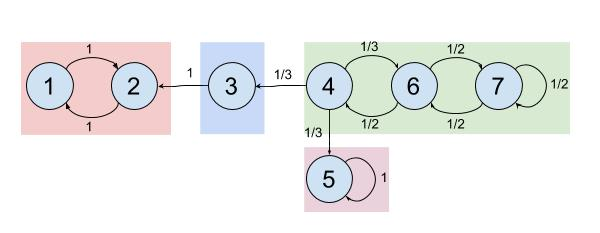
\includegraphics[scale=0.5]{ProbaTD8ex1.jpg}  

\subsection{Les classes transitoires et récurrentes :}
Cette chaîne de Markov comporte 2 classes transitoires et 2 classes récurrentes :
\begin{itemize}
\item Transitoires :
\begin{itemize}
\item $\{4,6,7\}$
\item $\{3\}$
\end{itemize}
\item Récurrentes :
\begin{itemize}
\item $\{1,2\}$
\item $\{5\}$
\end{itemize}
\end{itemize}

\section{Transmission de message}
\subsection*{Enoncé}
Un message pouvant prendre deux formes (état 1 ou état 2) est transmis de $A$ à $B$ en passant par $n$ intermédiaires. Chaque intermédiaire a une probabilité $p$ de transmettre correctement ce qu'il a reçu, $(1-p)$ de transmettre le message opposé. Soit $X_{k}$ le message transmis par le $k$-ième intermédiaire. 
\begin{enumerate}
\item Montrer que $X_{k}$ est une chaîne de Markov homogène, et calculer sa matrice de transition $G$.
\item Montrer que $G^{n}$ peut se mettre sous la forme $G_{1}+(2p-1)^{n}G_{2}$, avec
\begin{align*}
G_{1}=\frac{1}{2}\left(\begin{array}{cc}
 1 & 1\\
 1 & 1 \\
\end{array}\right)\\
G_{2}=\frac{1}{2}\left(\begin{array}{cc}
 1 & -1\\
 -1 & 1 \\
\end{array}\right)\\
\end{align*}
\item Calculer la probabilité pour que $B$ reçoive le message correct, et sa limite lorsque $n\rightarrow +\infty$
\end{enumerate}

\subsection{Montrer que $X_{k}$ est une chaîne de Markov homogène, et calculer sa matrice de transition $G$.}
La probabilité que le message soit dans dans un état ne dépend que de l'état précédent, ainsi on a pour tout $(i,j) \in \mathbb{N}^{2}$ et pour tout $(k_{1},k_{2}) \in \{1,2\}^{2}$ :
\[ P(X_{i+1}=k_{1}\mid X_{i}=k_{2}) = P(X_{j+1}=k_{1}\mid X_{j}=k_{2}) \]
La chaîne de Markov $X_{k}$ est donc homogène. On calcule maintenant sa matrice de transition $G$ :
\begin{align*}
G_{i,j} &= P(X_{1}=j\mid X_{0}=i)\\
G_{1,1} &= p\\
G_{1,2} &= 1-p\\
G_{2,1} &= 1-p\\
G_{2,2} &= p\\
G &= \left(\begin{array}{cc}
p & 1-p \\
1-p & p \\
\end{array}\right)\\
\end{align*}

\subsection{Montrer que $G^{n}$ peut se mettre sous la forme $G_{1}+(2p-1)^{n}G_{2}$}
On va réaliser une démonstration par récurrence, Soit $P_{n}$ la propriété : $G^{n}= G_{1}+(2p-1)^{n}G_{2}$:
\begin{itemize}
\item \textit{Initialisation} : On initialise à $n=1$ :
\begin{align*}
G^{1} &= \left(\begin{array}{cc}
p & 1-p \\
1-p & p \\
\end{array}\right)\\
G_{1}+(2p-1)^{1}G_{2} &= \frac{1}{2}\left(\begin{array}{cc}
 1 & 1\\
 1 & 1 \\
\end{array}\right) + (2p-1) \times \frac{1}{2}\left(\begin{array}{cc}
 1 & -1\\
 -1 & 1 \\
\end{array}\right)\\
&= \frac{1}{2}\left(\begin{array}{cc}
 1+2p-1 & 1-2p+1\\
 1-2p+1 & 1+2p-1 \\
\end{array}\right)\\
&= \frac{1}{2}\left(\begin{array}{cc}
 2p & 2-2p\\
 2-2p & 2p \\
\end{array}\right)\\
&= \left(\begin{array}{cc}
 p & 1-p\\
 1-p & p \\
\end{array}\right)\\
G_{1}+(2p-1)^{1}G_{2} &= G^{1}\\
\end{align*}
La propriété $P_{1}$ est vérifiée.
\item \textit{Récurrence} : On suppose que $P_{n}$ est vérifiée et on cherche à montrer que $P_{n+1}$ l'est aussi :
\begin{align*}
G^{n+1} =& G \times G^{n}\\
=&  \left(\begin{array}{cc}
p & 1-p \\
1-p & p \\
\end{array}\right) \times \frac{1}{2} \left(\left(\begin{array}{cc}
1 & 1 \\
1 & 1 \\
\end{array}\right) + (2p-1)^{n}  \left(\begin{array}{cc}
1 & -1 \\
-1 & 1 \\
\end{array}\right)\right)\\
=& \frac{1}{2}  \left(\begin{array}{cc}
p & 1-p \\
1-p & p \\
\end{array}\right) \times  \left(\begin{array}{cc}
1 & 1 \\
1 & 1 \\
\end{array}\right) + \\
&\frac{1}{2}(2p-1)^{n}  \left(\begin{array}{cc}
p & 1-p \\
1-p & p \\
\end{array}\right) \times  \left(\begin{array}{cc}
1 & -1 \\
-1 & 1 \\
\end{array}\right)\\
=&\frac{1}{2} \left(\left(\begin{array}{cc}
p+1-p & p+1-p \\
1-p+p & 1-p+p \\
\end{array}\right) + (2p-1)^{n}  \left(\begin{array}{cc}
p-1+p & -p+1-p \\
1-p-p & -1+p+p \\
\end{array}\right)\right)\\
=& \frac{1}{2} \left(  \left(\begin{array}{cc}
1 & 1 \\
1 & 1 \\
\end{array}\right) + (2p-1)^{n}  \left(\begin{array}{cc}
2p-1 & -(2p-1) \\
-(2p-1) & 2p-1 \\
\end{array}\right)\right)\\
=&\frac{1}{2}+(2p-1)^{n+1} \left(\begin{array}{cc}
1 & -1 \\
-1 & 1 \\
\end{array}\right)\\
G^{n+1} =& G_{1}+(2p-1)^{n+1}G_{2}\\
\end{align*}
Si $P_{n}$ est vérifiée alors $P_{n+1}$ l'est aussi. $P_{n}\Rightarrow P_{n+1}$.
\item \textit{Conclusion} : On a donc $P_{1}$ est vrai et $P_{n}\Rightarrow P_{n+1}$ ainsi par récurrence on obtient $P_{n}$ est vrai pour tout $n\geqslant 1$
\end{itemize}

\subsection{Calculer la probabilité pour que $B$ reçoive le message correct, et sa limite lorsque $n\rightarrow +\infty$}
On cherche $P(X_{n}=1)$. On calcule tout d'abord $G^{n}$ :
\begin{align*}
G^{n} =& G_{1}+(2p-1)^{n}G_{2}\\
=& \frac{1}{2}\left(\begin{array}{cc}
 1 & 1\\
 1 & 1 \\
\end{array}\right) + (2p-1)^{n} \times \frac{1}{2}\left(\begin{array}{cc}
 1 & -1\\
 -1 & 1 \\
\end{array}\right)\\
=& \frac{1}{2}\left(\begin{array}{cc}
 1+(2p-1)^{n} & 1-(2p-1)^{n}\\
 1-(2p-1)^{n} & 1+(2p-1)^{n} \\
\end{array}\right)
\end{align*}
On sait que le message est dans le bon état avant la première transmission ainsi $X_{0}=1$
\begin{align*}
P(X_{n}=1) &= P(X_{n}=1\mid X_{0}=1)\\
&= (G^{n})_{1,1}\\
&= \frac{1}{2}\left(1+(2p-1)^{n}\right)\\
\end{align*}
Comme $0\leqslant p \leqslant 1$ on a $|2p-1|\leqslant 1$ ainsi on distingue trois cas différents pour calculer la limite lorsque $n\rightarrow +\infty$ :
\begin{itemize}
\item $p=1$ :
\begin{align*}
P(X_{n}=1) &= \frac{1}{2}(1+1^{n})\\
&= 1\\
\lim\limits_{n\rightarrow+\infty} P(X_{n}=1) &= 1\\
\end{align*}
\item $p=0$
\begin{align*}
P(X_{n}=1) &= \frac{1}{2}(1+(-1)^{n})\\
\end{align*}
Dans ce cas $P(X_{n}=1)$ n'admet pas de limite quand $n\rightarrow +\infty$. Cela dépend de la parité de $n$.
\item $0<p<1$ : dans ce cas $|2p-1|< 1$ ainsi $\lim\limits_{n\rightarrow+\infty} (2p-1)^{n} = 0$ :
\begin{align*}
P(X_{n}=1) &= \frac{1}{2}(1+(2p-1)^{n})\\
&= 1\\
\lim\limits_{n\rightarrow+\infty} P(X_{n}=1) &= \frac{1}{2} + \lim\limits_{n\rightarrow+\infty} \frac{(2p-1)^{n}}{2}\\
\lim\limits_{n\rightarrow+\infty} P(X_{n}=1) &= \frac{1}{2}\\
\end{align*}
\end{itemize}

\section{Modèle élémentaire de gestion de stock}
\subsection*{Enoncé}
La demande d'un bien entre les instants $n$ et $n+1$ est représentée par une variable aléatoire positive $Y_{n+1}$. Le niveau du stock du bien est égal $X_{n}$ à l'instant $n$. La gestion du stock se fait de la manière suivante :
\begin{itemize}
\item si $X_{n}-Y_{n+1}\geqslant m$, alors le stock n'est pas réapprovisionné, et $X_{n+1} = X_{n}-Y_{n+1}$.
\item si $X_{n}-Y_{n+1}<m$, alors le stock est réapprovisionné et porté au niveau $M$ : $X_{n+1}=M$
\end{itemize}
On suppose que $X_{0}$ est de loi quelconque sur $\{m,\ldots,M\}$, et que les $(Y_{n})_{n\in\mathbb{N}}$ et $X_{0}$ sont indépendantes. Pour l'application numérique on pose que les $(Y_{n})_{n\in\mathbb{N}}$ suivent une loi indépendante sur $\{0,1,2\}$, et que $M=3$ et $m=1$.

\subsection{Montrer que $X_{n}$ est une chaîne de Markov homogène et calculer la matrice de transition $G$}
Les probabilités des événements de l'état $X_{n}$ ne dépendent que de l'état précédent $X_{n+1}$ et d'une variable $Y_{n}$ indépendante. $X_{n}$ est donc une chaîne de Markov homogène. $X_{n}$ ne peut prendre que des valeurs qu'entre $n$ et $m$ soit entre $1$ et $3$.
\begin{align*}
P(X_{1}=1\mid X_{0}=1) =& P(Y_{0} = 0) & P(X_{1}=1\mid X_{0}=2) =& P(Y_{0} = 1)\\
=& \frac{1}{3} & =& \frac{1}{3}\\
P(X_{1}=1 \mid X_{0}=3) =& P(Y_{0} = 2)\\
=& \frac{1}{3} \\
\\
P(X_{1}=2\mid X_{0}=1) =& P(Y_{0} = -1) & P(X_{1}=2\mid X_{0}=2) =& P(Y_{0} = 0)\\
=& 0 & =& \frac{1}{3}\\
P(X_{1}=2\mid X_{0}=3) =& P(Y_{0} = 1)\\
=& \frac{1}{3} \\
\\
P(X_{1}=3\mid X_{0}=1) =& P(Y_{0} > 1) & P(X_{1}=3\mid X_{0}=2) =& P(Y_{0} > 2)\\
=& P(Y_{0}=2) + P(Y_{0}=3) & =& P(Y_{0}=3)\\
=& \frac{2}{3} & =& \frac{1}{3}\\
P(X_{1}=3\mid X_{0}=3) =& P(Y_{0} = 0)\\
=& \frac{1}{3} \\
\end{align*}
On trouve donc la matrice $G$, suivante :
\[ G=\frac{1}{3}\left(\begin{array}{ccc}
1 & 0 & 2\\
1 & 1 & 1\\
1 & 1 & 1\\
\end{array}\right)\]

\subsection{Trouver la probabilité invariante $\nu$. Quelle est la probabilité en régime stationnaire d'être en rupture de stock ?}
On cherche la fonction de masse $\nu$ dont la notation vectorielle vérifie la propriété suivante :
\begin{align*}
\nu =& \nu G\\
=& \frac{1}{3}\left(\nu_{1},\nu_{2},\nu_{3}\right) \left(\begin{array}{ccc}
1 & 0 & 2\\
1 & 1 & 1\\
1 & 1 & 1\\
\end{array}\right)\\
\left(\nu_{1},\nu_{2},\nu_{3}\right)=& \frac{1}{3}\left(\nu_{1}+\nu_{2}+\nu_{3}, \nu_{2}+\nu_{3}, 2\nu_{1}+\nu_{2}+\nu_{3}\right)\\
\end{align*}
On en déduit le système d'équations suivant :
\begin{align*}
& \left\lbrace \begin{array}{rcl}
\nu_{1} &=& \frac{1}{3}(\nu_{1}+\nu_{2}+\nu_{3})\\
\nu_{2} &=& \frac{1}{3}(\nu_{2}+\nu_{3})\\
\nu_{3} &=& \frac{1}{3}(2\nu_{1}+\nu_{2}+\nu_{3})\\
\end{array}\right.\\
\Leftrightarrow & \left\lbrace \begin{array}{rcl}
3\nu_{1} &=& \nu_{1}+\nu_{2}+\nu_{3}\\
3\nu_{2} &=& \nu_{2}+\nu_{3}\\
3\nu_{3} &=& 2\nu_{1}+\nu_{2}+\nu_{3}\\
\end{array}\right.\\
\Leftrightarrow & \left\lbrace \begin{array}{rcl}
2\nu_{1} &=& \nu_{2}+\nu_{3}\\
2\nu_{2} &=& \nu_{3}\\
2\nu_{3} &=& 2\nu_{1}+\nu_{2}\\
\end{array}\right.\\
\Leftrightarrow & \left\lbrace \begin{array}{rcl}
2\nu_{1} &=& 3\nu_{2}\\
2\nu_{2} &=& \nu_{3}\\
4\nu_{2} &=& 2\nu_{1}+\nu_{2}\\
\end{array}\right.\\
\Leftrightarrow & \left\lbrace \begin{array}{rcl}
\nu_{1} &=& \frac{3}{2}\nu_{2}\\
2\nu_{2} &=& \nu_{3}\\
3\nu_{2} &=& 2\times\frac{3}{2}\nu_{1}\\
\end{array}\right.\\
\Leftrightarrow & \left\lbrace \begin{array}{rcl}
\nu_{1} &=& \frac{3}{2}\nu_{2}\\
\nu_{3} &=& 2\nu_{2}\\
\nu_{2} &=& \nu_{2}\\
\end{array}\right.\\
\end{align*}
Les trois équations n'étaient pas indépendantes, nous avons donc une infinité de solutions à ce système mais nous connaissons une contrainte supplémentaire sur $\nu$, en tant que fonction de masse la somme de ses valeurs doit donner 1. Nous avons donc l'équation supplémentaire suivante $\nu_{1}+\nu_{2}+\nu_{3}=1$ :
\renewcommand\arraystretch{1.2}
\begin{align*}
& \left\lbrace \begin{array}{rcl}
\nu_{1} &=& \frac{3}{2}\nu_{2}\\
\nu_{3} &=& 2\nu_{2}\\
\nu_{1}+\nu_{2}+\nu_{3} &=& 1
\end{array}\right.\\
\Leftrightarrow & \left\lbrace \begin{array}{rcl}
\nu_{1} &=& \frac{3}{2}\nu_{2}\\
\nu_{3} &=& 2\nu_{2}\\
\left(\frac{3}{2}+1+2\right)\nu_{2} &=& 1
\end{array}\right.\\
\Leftrightarrow & \left\lbrace \begin{array}{rcl}
\nu_{1} &=& \frac{3}{9}\\
\nu_{3} &=& \frac{4}{9}\\
\nu_{2} &=& \frac{2}{9}
\end{array}\right.\\
\Leftrightarrow & \left\lbrace \begin{array}{rcl}
\nu_{1} &=& \frac{1}{3}\\
\nu_{3} &=& \frac{4}{9}\\
\nu_{2} &=& \frac{2}{9}
\end{array}\right.\\
\end{align*}
\renewcommand\arraystretch{1}
Nous avons donc trouvé la loi de probabilité invariante $\nu=\left(\frac{1}{3},\frac{4}{9},\frac{2}{9}\right)$. Nous cherchons maintenant la probabilité de tomber en rupture de stock selon cette loi. Une rupture de stock apparaît lorsque $Y_{n}>X_{n}$ or cela n'est possible que si $X_{n}=1$ et $Y_{n}=2$. On calcule donc $P(X_{n}=1 \cap Y_{n}=2)$ avec $X_{n}$ suivant la loi invariante $\nu$ :
\begin{align*}
P(X_{n}=1 \cap Y_{n}=2)=& P(X_{n}=1) \times P(Y_{n}=2) & \text{car }X_{n}\text{ et }Y_{n}\text{ indépendantes}\\
=& \frac{1}{3} \times \frac{1}{3}\\
P(X_{n}=1 \cap Y_{n}=2)=& \frac{1}{9}
\end{align*}
Avec cette organisation on risque de tomber en rupture de stock 1 jour sur 9
\end{document}